% !TeX root = main.tex
\chapter{The Gemmini DNN Accelerator: An Architectural Overview}
\label{chap:gemmini_overview}

As established in the previous chapter, the System-on-Chip (SoC) developed in this thesis utilizes a single \texttt{Rocket} Core augmented with a specialized accelerator for deep learning workloads. This chapter delves into the architecture of this accelerator: \texttt{Gemmini}, a sophisticated component designed to overcome the fundamental limitations of general-purpose processors for Deep Neural Network (DNN) tasks.

\begin{figure}[htbp]
    \centering
    
\includegraphics[width=0.9\textwidth]{Gemmini_Logo.pdf}
    \caption{Gemmini Logo. Source: \cite{gemini-dac}.}
    \label{fig:gemmini_logo}
\end{figure}

\section{Introduction: The Full-Stack Accelerator Philosophy}
\label{sec:gemmini_intro}

\texttt{Gemmini} is an open-source, full-stack DNN accelerator \textit{generator} developed at the University of California, Berkeley \cite{gemini-dac}. It is designed not merely as a standalone hardware component, but as a complete ecosystem for exploring and evaluating domain-specific hardware acceleration. 

Its design is rooted in the philosophy of "full-stack" evaluation. Many accelerators are designed and tested in isolation, which fails to account for critical system-level effects such as memory bus contention, cache coherency overhead, and operating system interactions (e.g., page faults and context switches) \cite{gemini-dac}. By generating not only the accelerator RTL but also a complete, Linux-capable SoC using the \texttt{Chipyard} framework, \texttt{Gemmini} enables a comprehensive analysis of these cross-stack interactions. This allows for a more realistic assessment of real-world performance and energy efficiency \cite{gemini-dac}.

Crucially, as a generator written in Chisel, \texttt{Gemmini} is not a single, fixed hardware design. As illustrated in Figure \ref{fig:gemmini_flexibility}, its flexible template can be configured to produce a wide spectrum of systolic architectures, from highly pipelined designs to parallel-vector engines. This makes it an exceptionally powerful platform for the academic exploration of accelerator architectures.

For this thesis, leveraging \texttt{Gemmini} provides the opportunity to explore a powerful DNN accelerator within a realistic SoC environment.

\begin{figure}[h!]
    \centering
    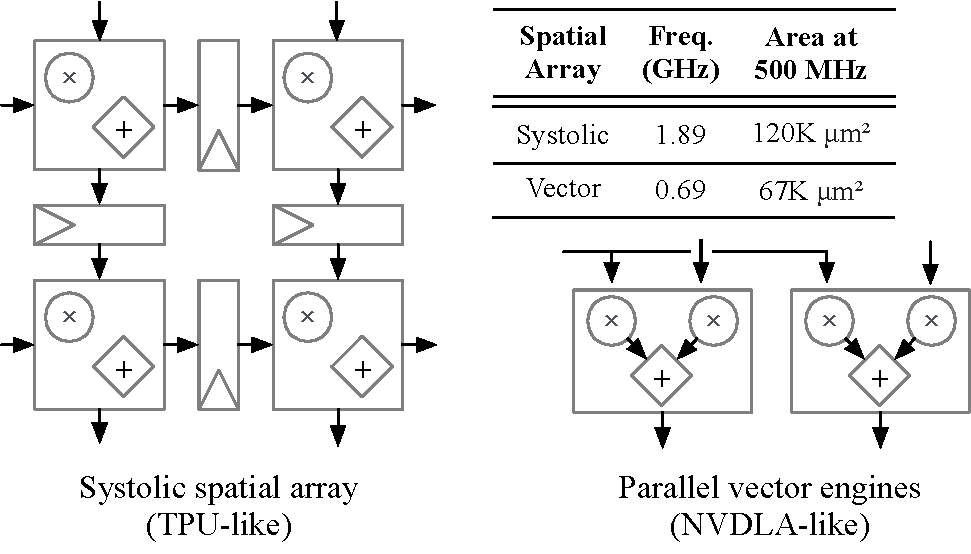
\includegraphics[width=0.9\textwidth]{Gemmini_SystolicNVDLA.pdf} 
    \caption[Architectural Flexibility of the Gemmini Generator]{The design space enabled by the Gemmini generator, allowing it to produce a wide variety of spatial array structures. Source: \cite{gemini-dac}.}
    \label{fig:gemmini_flexibility}
\end{figure}

\section{Top-Level Architectural Blueprint}
\label{sec:gemmini_blueprint}
The \texttt{Gemmini} generator can produce a wide range of accelerator instances based on a flexible architectural template. To understand the \texttt{Gemmini} architecture, we first examine the high-level template shown in Figure \ref{fig:gemmini_template}. This blueprint illustrates the three primary components of the accelerator---the Controller, the on-chip memory (Scratchpad and Accumulator), and the compute core (Spatial Array)---and their interface with the host CPU and system DRAM. The following sections provide a detailed analysis of each of these blocks.

\begin{figure}[htbp]
    \centering
    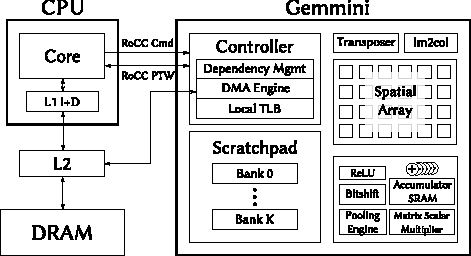
\includegraphics[width=0.9\textwidth]{Gemmini_ArchitectureOverview.pdf}
    \caption{High-level overview of the Gemmini accelerator template integrated with a host CPU and system memory hierarchy. Source: \cite{gemini-dac}.}
    \label{fig:gemmini_template}
\end{figure}

\section{Analysis of Core Architectural Components}
\label{sec:gemmini_components}

\subsection{The Systolic Compute Engine}
The computational heart of \texttt{Gemmini} is its systolic array, a highly configurable spatial array that functions as a powerful General Matrix-Matrix Multiplication (GEMM) engine. The array's microarchitecture, as detailed in Figure \ref{fig:gemmini_microarch}, features a two-level hierarchy composed of \texttt{Tiles} and individual Processing Elements (PEs). Each PE is capable of performing a Multiply-Accumulate (MAC) operation in a single clock cycle. This hierarchical and configurable design allows \texttt{Gemmini} to efficiently execute the dense matrix multiplications fundamental to modern Deep Neural Networks (DNNs).

\begin{figure}[htbp]
    \centering
    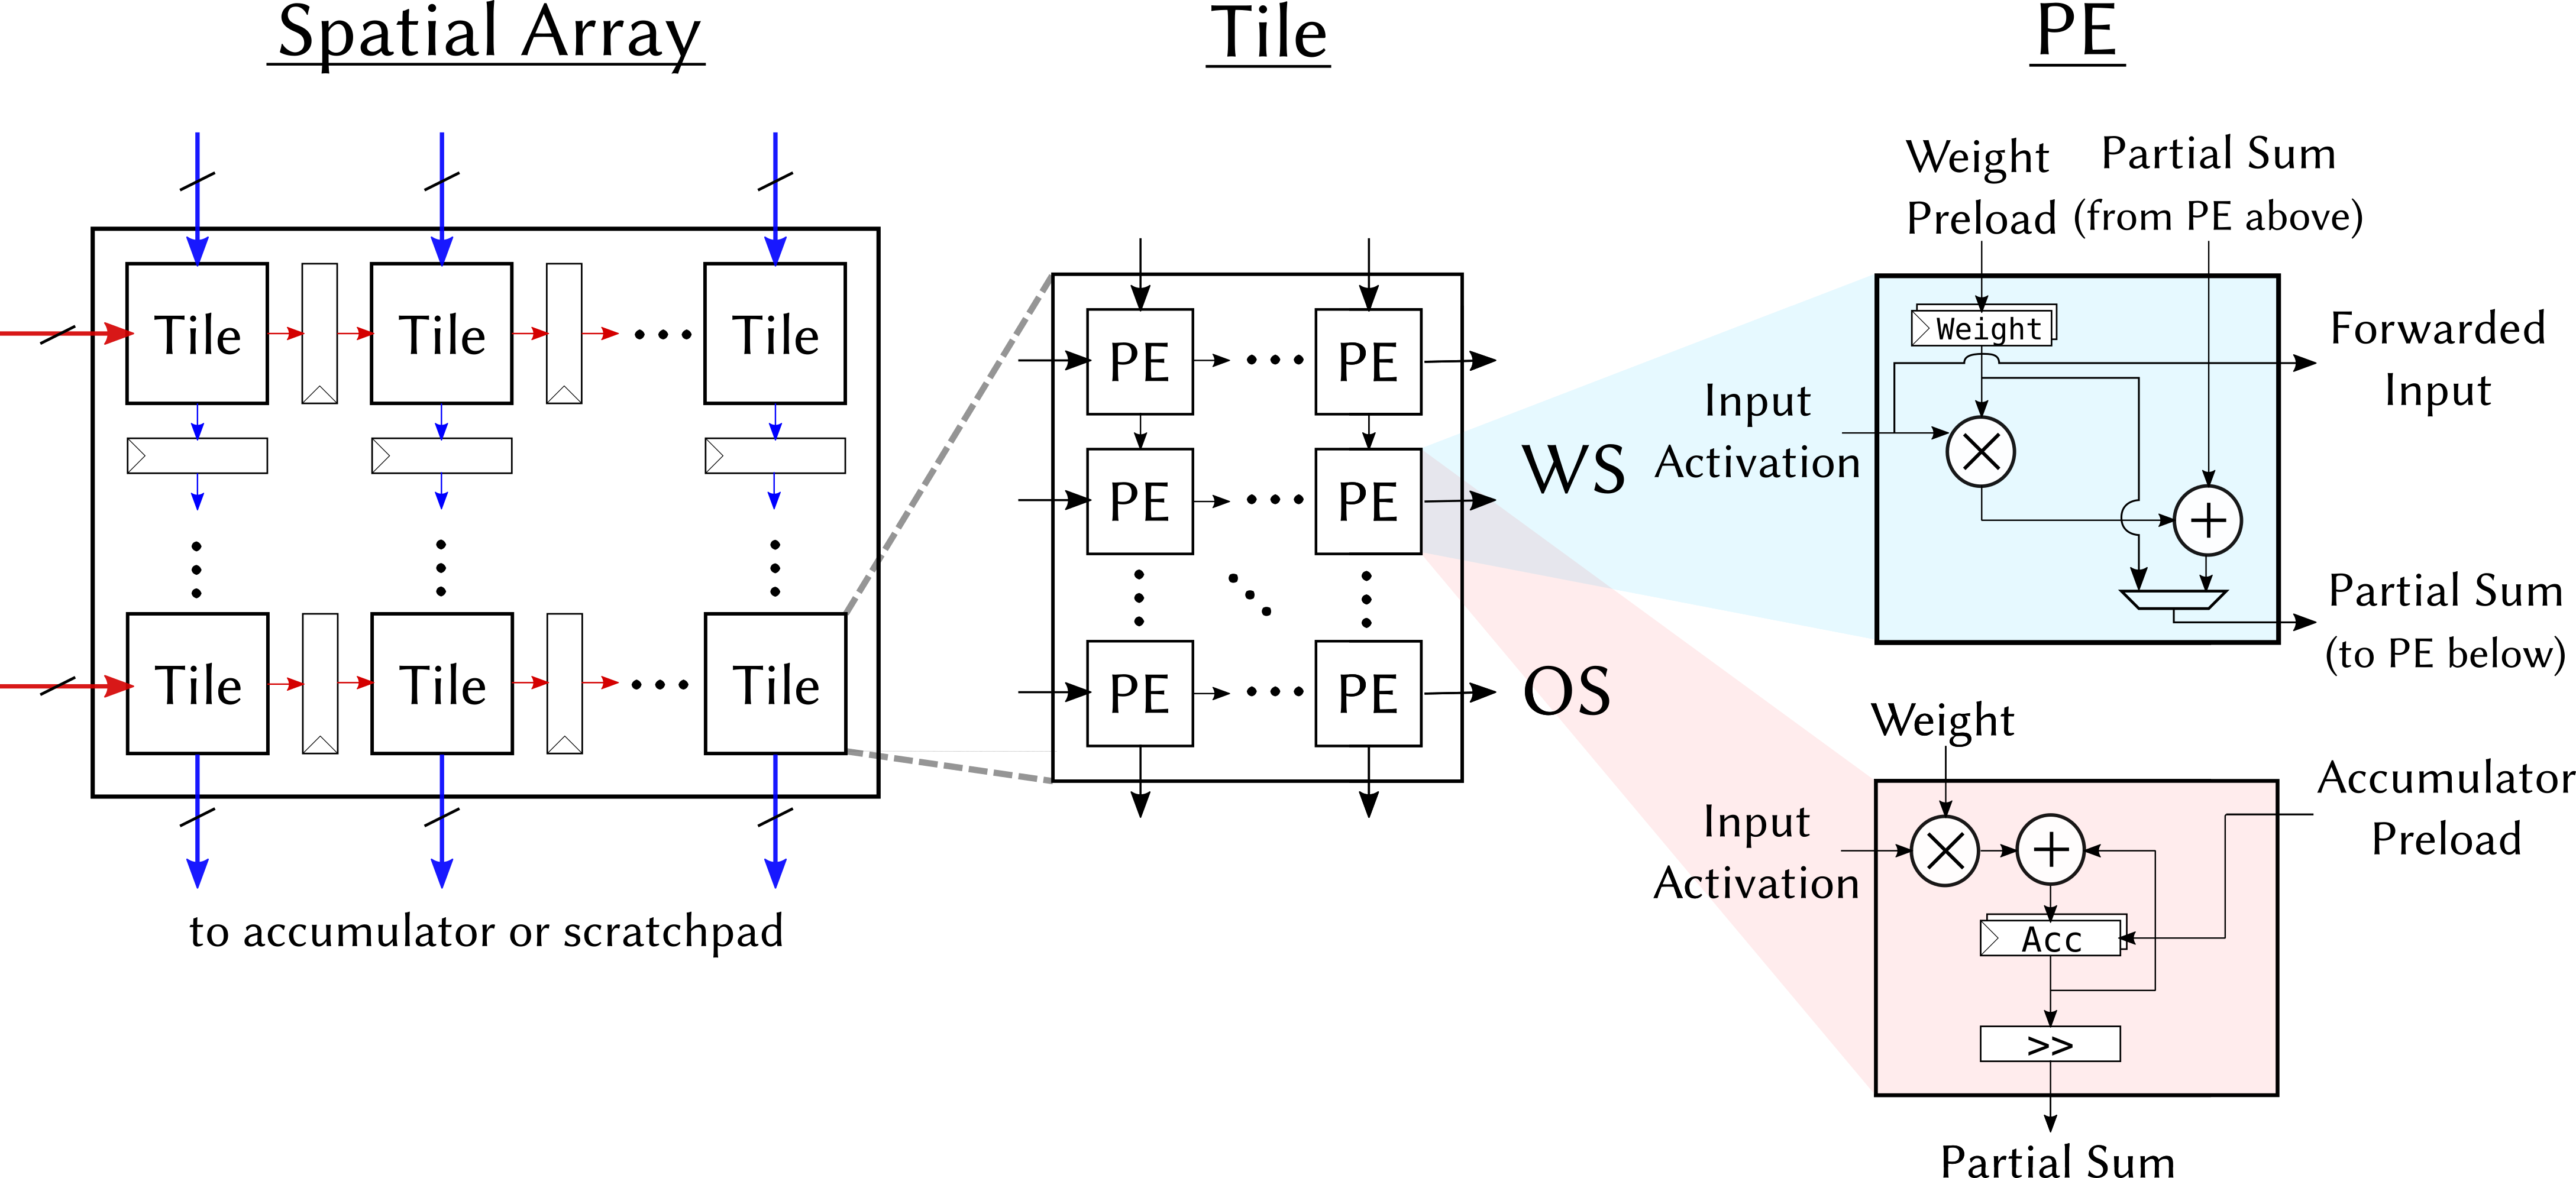
\includegraphics[width=0.8\textwidth]{Gemmini_MicroArchitecture.png}
    \caption[Microarchitecture of Gemmini's Spatial Array]{The two-level hierarchy of Gemmini's spatial array, composed of tiles and Processing Elements (PEs). Source: \cite{gemini-dac}.}
    \label{fig:gemmini_microarch}
\end{figure}

The key parameters of the systolic array can be specified at generation time:
\begin{itemize}
    \item \textbf{Dimensions:} The size of the PE grid, structured into a hierarchy of tiles, can be configured (e.g., a 16x16 array composed of 2x2 tiles, each with 8x8 PEs). This allows for a trade-off between hardware area and parallel processing capability.
    \item \textbf{Dataflow:} \texttt{Gemmini} primarily supports two dataflow strategies: Weight Stationary (WS) and Output Stationary (OS). 
    \begin{itemize}
        \item In \textbf{WS dataflow}, the DNN weights are pre-loaded into the PEs and remain stationary, maximizing weight reuse as input activations are streamed through. 
        \item In \textbf{OS dataflow}, partial sums of the output activations remain stationary within the PEs, while both inputs and weights are streamed. This is particularly beneficial for layers with low weight reuse.
    \end{itemize}
    The choice of dataflow has a significant impact on performance and energy efficiency.
    \item \textbf{Pipelining:} The degree of pipelining within the array and its PEs can be configured, affecting the maximum clock frequency and overall throughput.
\end{itemize}

\subsubsection{Mapping Convolution to Hardware: The \texttt{im2col} Transformation}
\label{subsubsec:im2col}
While systolic arrays are fundamentally designed to accelerate General Matrix-Matrix Multiplication (GEMM), they are adept at accelerating 2D convolutions through a crucial data-restructuring technique known as \texttt{im2col} ("image-to-column"). This process unrolls the overlapping input image patches from a convolutional layer into the columns of a new, larger matrix. As shown in Figure \ref{fig:im2col}, this new matrix can then be multiplied with a corresponding weight matrix, effectively \textbf{converting the convolution into a GEMM operation} that the systolic array can process with maximum efficiency.

Recognizing the computational cost of this pre-processing step, \texttt{Gemmini} can be configured with a dedicated hardware unit to perform the \texttt{im2col} transformation on-the-fly. This offloads the data restructuring from the host CPU, freeing it for other tasks and streamlining the overall computation pipeline. The decision to include this unit represents a classic area-versus-performance trade-off in the accelerator design.

\begin{figure}[h!]
    \centering
    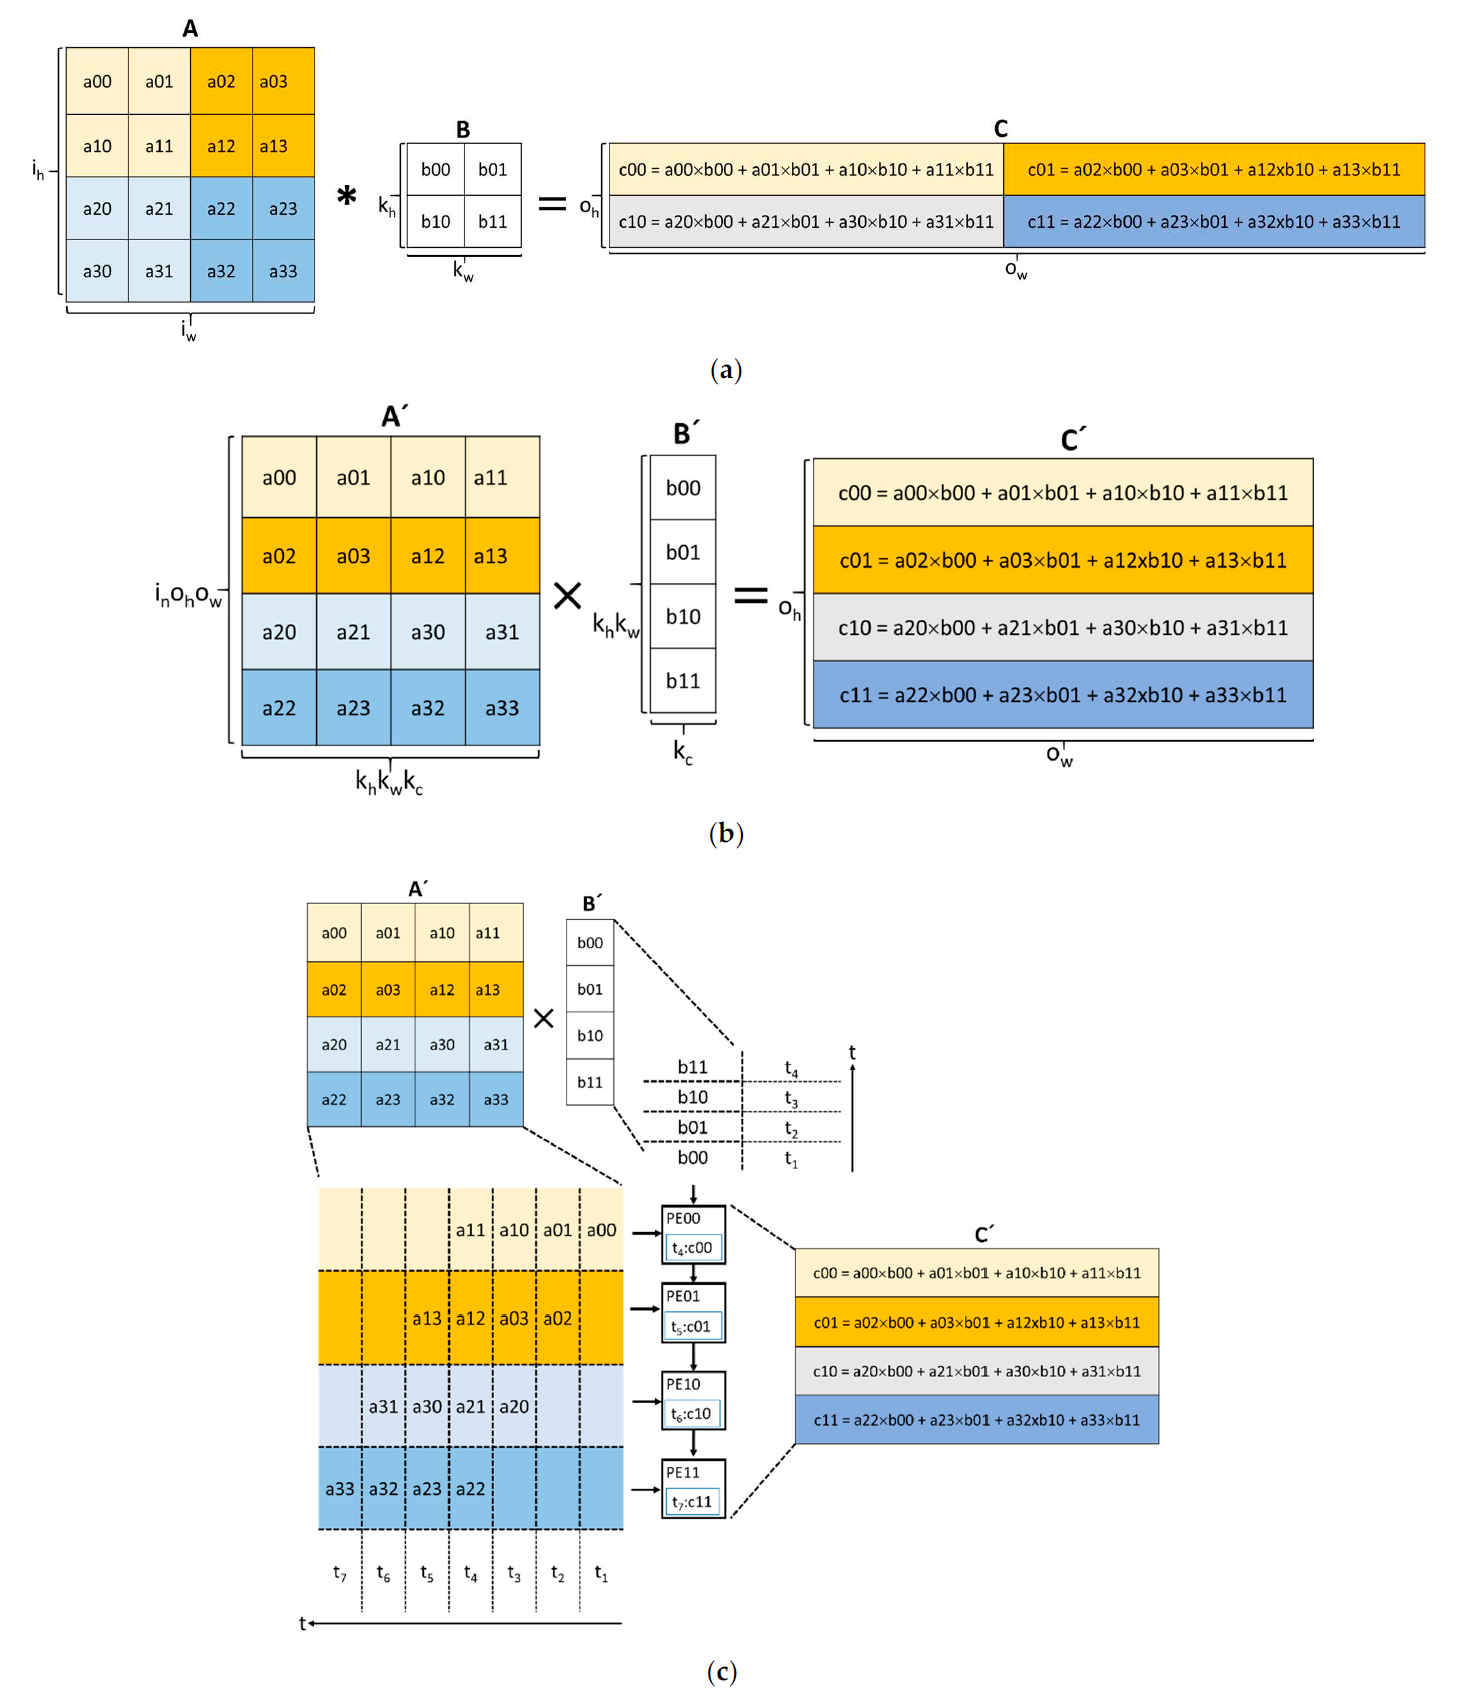
\includegraphics[width=\textwidth]{Gemmini_Im2Col.png}
    \caption[The im2col Transformation]{From convolution to systolic array computation: (a) direct convolution operation; (c) example of a systolic array operation; (b) A visualization of the \texttt{im2col}-based GEMM operation. The 3D input tensor (left) is transformed into a 2D matrix (center) that can be processed by the systolic array. Adapted from Gookyi et al. \cite{gookyi2023gemmini_case_study}.}
    \label{fig:im2col}
\end{figure}


\subsection{The On-Chip Memory Subsystem}
To feed its high-throughput systolic array, \texttt{Gemmini} includes a specialized on-chip memory system. This design represents a deliberate trade-off between hardware-managed caches and software-managed memories.
\begin{itemize}
    \item \textbf{Scratchpad Memory:} A software-managed SRAM used for staging input activations, weights, and intermediate feature maps close to the systolic array. Its purpose is to reduce the latency and energy consumption associated with fetching data from higher levels of the memory hierarchy, such as the shared L2 cache or main memory (DRAM). Its capacity and banking are configurable.
    \item \textbf{Accumulator Memory:} Separate from the main scratchpad, \texttt{Gemmini} features a dedicated memory to store the partial sums generated by the MAC operations. This memory typically uses a higher precision data type (e.g., 32-bit integers) than the input data (e.g., 8-bit integers) to maintain accuracy during accumulation.
\end{itemize}

\section{SoC Integration and System-Level Features}
\label{sec:gemmini_integration}

\subsection{The RoCC Coprocessor Interface}
\texttt{Gemmini} integrates into the \texttt{Chipyard} SoC via the \textbf{Rocket Custom Coprocessor (RoCC)} interface. As a tightly-coupled coprocessor, it receives custom RISC-V instructions dispatched directly by the host \texttt{Rocket} Core's pipeline. This allows for low-latency command and control.



This integration uses a decoupled access-execute model, as illustrated conceptually in Figure~\ref{fig:decoupled_pipelines}. The host CPU issues three main types of commands to \texttt{Gemmini}: load (from main memory to scratchpad), execute (perform computation on data within the scratchpad), and store (from scratchpad to main memory). These commands are placed into separate hardware queues, allowing \texttt{Gemmini}'s internal controller then processes these commands asynchronously, and Gemmini's DMA engine to handle data movement in parallel with the systolic array's computations. This overlapping of communication and computation is crucial for hiding memory latency and maximizing the utilization of the systolic array.

\begin{figure}[htbp]
    \centering
    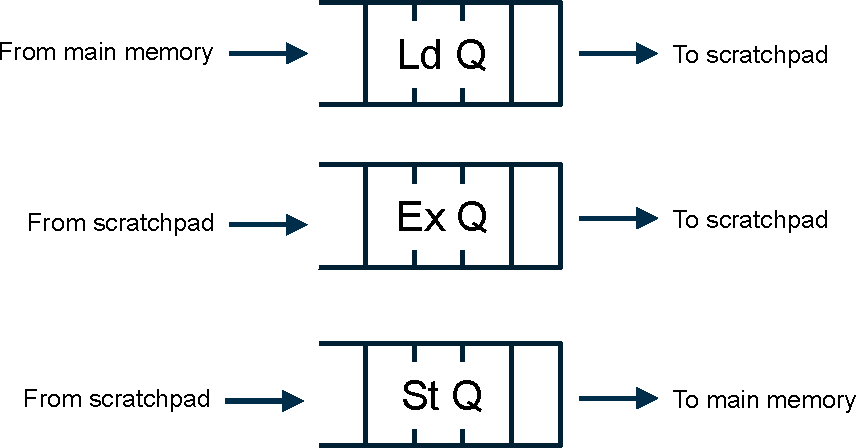
\includegraphics[width=0.8\textwidth]{Gemmini_DecoupledAccessExecutePipeline.pdf}
    \caption{Conceptual view of Gemmini's decoupled access-execute pipelines, managed by separate hardware command queues for Load, Execute, and Store operations. Source: \cite{gemini-dac}.}
    \label{fig:decoupled_pipelines}
\end{figure}

\subsection{Virtual Memory Support}
To operate correctly under a full-featured operating system like Linux, an accelerator's DMA engine must be able to translate virtual memory addresses into physical addresses. \texttt{Gemmini} is designed with this "full-stack" capability. It can be configured to share the host CPU's Page Table Walker (PTW) to perform its own address translations, and it includes its own local Translation Lookaside Buffer (TLB) to cache these translations and reduce latency.

\section{Summary}
\label{sec:gemmini_overview_summary}
In summary, \texttt{Gemmini} is a sophisticated, highly configurable DNN accelerator generator that embodies the principles of systolic computation. Its key architectural features include a powerful systolic array, a specialized on-chip memory hierarchy, and a tightly-coupled integration with a host processor via the \texttt{RoCC} interface, including support for system-level features like virtual memory. This design enables the high-performance execution of DNN workloads within a full-stack, system-level context. 

Having established this architectural overview, the following chapter will now perform a deep dive into the specifics of \texttt{Gemmini}'s internal command processing and its multi-level programming model.